\documentclass[11pt]{article}
\usepackage[margin=0.75in]{geometry}
\usepackage{amsmath}
\usepackage{tikz}
\usepackage{tcolorbox}
\usetikzlibrary{patterns}
\usetikzlibrary{arrows.meta}

\title{WARP Violation: Different Danger Zone Scenarios}
\author{Complete Visual Guide}
\date{February 28, 2026}

\begin{document}

\maketitle

\section{Overview}

The WARP violation "danger zone" is defined by TWO inequalities:
\begin{enumerate}
\item \textbf{Old budget constraint:} $p_1^{old} x_1 + p_2^{old} x_2 \leq m$ (was affordable before)
\item \textbf{New iso-cost constraint:} $p_1^{new} x_1 + p_2^{new} x_2 \geq C$ (costs enough now)
\end{enumerate}

The shape and existence of the danger zone depends on:
\begin{itemize}
\item The slope of each line
\item Where they intersect (if at all)
\item The relative price changes
\end{itemize}

Let's explore different scenarios!

\newpage

\section{Scenario 1: Triangle Touching x-axis (Classic Case)}

\textbf{Setup:}
\begin{itemize}
\item Old prices: $(1, 3)$, bought $(4, 2)$, budget = 10
\item New prices: $(3, 5)$, old bundle costs 22
\end{itemize}

\begin{center}
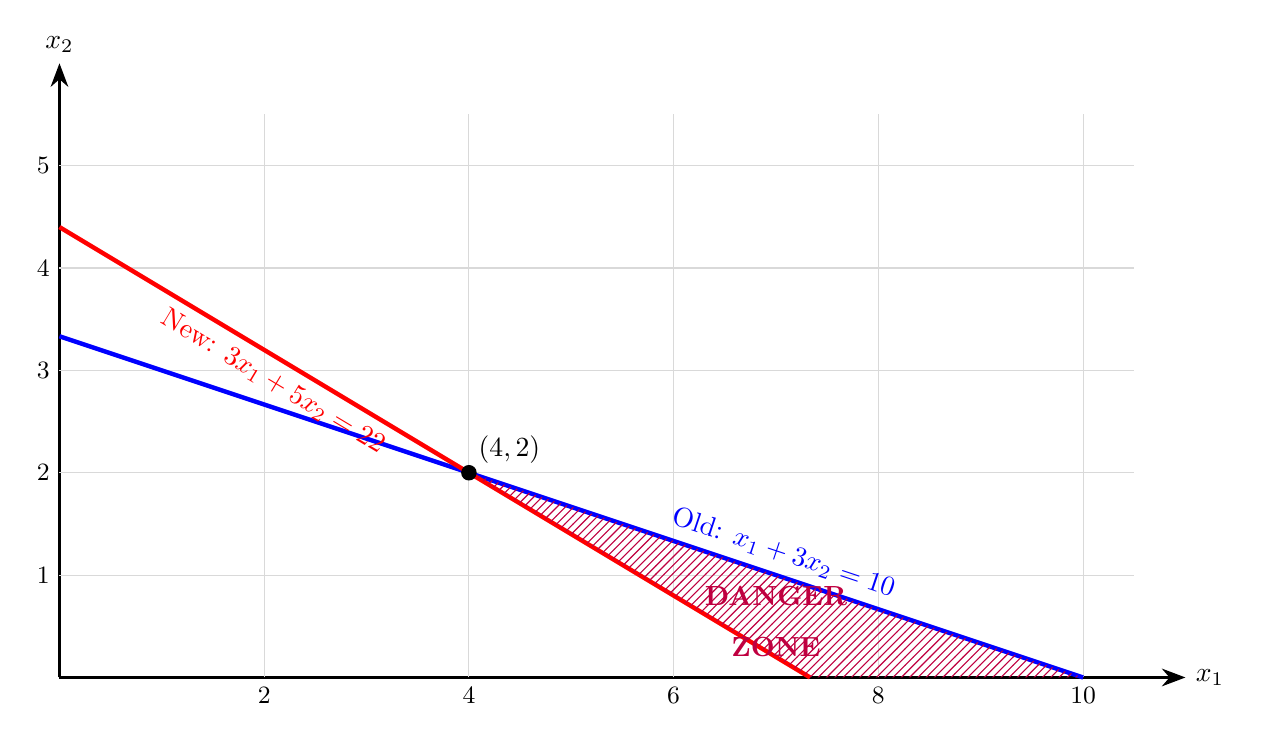
\begin{tikzpicture}[scale=1.3]
    \draw[-{Stealth[length=3mm]},thick] (0,0) -- (11,0) node[right] {$x_1$};
    \draw[-{Stealth[length=3mm]},thick] (0,0) -- (0,6) node[above] {$x_2$};

    \foreach \x in {2,4,6,8,10}
        \draw[gray!30] (\x,0) -- (\x,5.5);
    \foreach \y in {1,2,3,4,5}
        \draw[gray!30] (0,\y) -- (10.5,\y);

    \draw[blue, ultra thick] (0,3.333) -- (10,0) node[pos=0.7,above,sloped,blue] {Old: $x_1 + 3x_2 = 10$};
    \draw[red, ultra thick] (0,4.4) -- (7.333,0) node[pos=0.3,below,sloped,red] {New: $3x_1 + 5x_2 = 22$};

    \fill[pattern=north east lines, pattern color=purple] (4,2) -- (7.333,0) -- (10,0) -- cycle;

    \filldraw[black] (4,2) circle (2pt) node[above right] {$(4,2)$};

    \node[purple, font=\bfseries] at (7,0.8) {DANGER};
    \node[purple, font=\bfseries] at (7,0.3) {ZONE};

    \foreach \x in {2,4,6,8,10}
        \node[below] at (\x,0) {\small \x};
    \foreach \y in {1,2,3,4,5}
        \node[left] at (0,\y) {\small \y};
\end{tikzpicture}
\end{center}

\textbf{Characteristics:}
\begin{itemize}
\item Triangle shape
\item One vertex at original bundle $(4,2)$
\item Two vertices on $x_1$-axis
\item This happens when: old budget line is \textbf{steeper} than new iso-cost line
\end{itemize}

\newpage

\section{Scenario 2: Triangle NOT Touching x-axis}

\textbf{Setup:}
\begin{itemize}
\item Old prices: $(2, 1)$, bought $(3, 4)$, budget = 10
\item New prices: $(1, 3)$, old bundle costs 15
\end{itemize}

\begin{center}
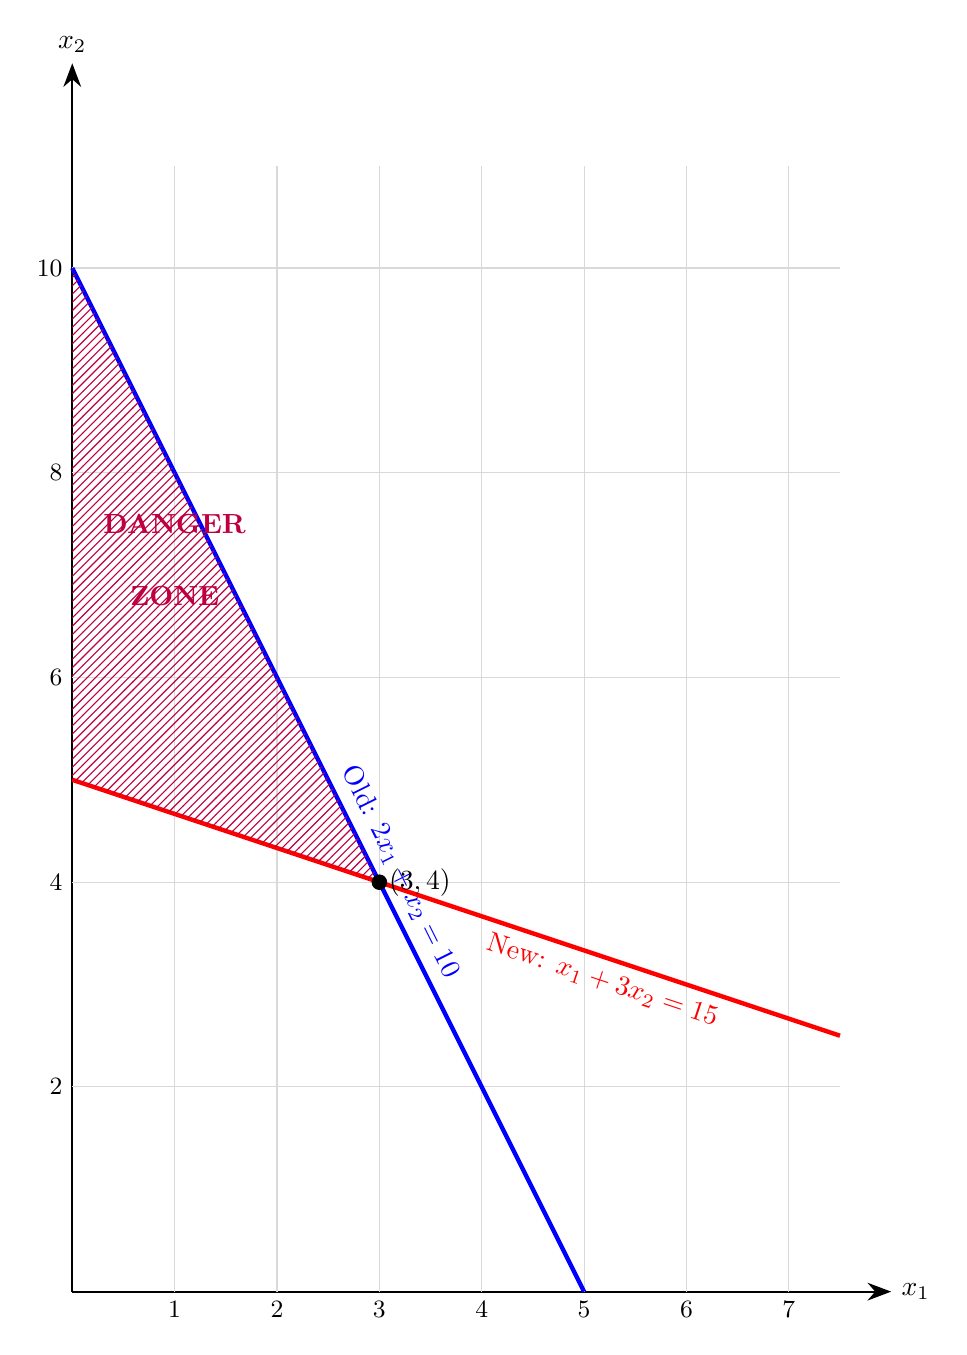
\begin{tikzpicture}[scale=1.3]
    \draw[-{Stealth[length=3mm]},thick] (0,0) -- (8,0) node[right] {$x_1$};
    \draw[-{Stealth[length=3mm]},thick] (0,0) -- (0,12) node[above] {$x_2$};

    \foreach \x in {1,2,3,4,5,6,7}
        \draw[gray!30] (\x,0) -- (\x,11);
    \foreach \y in {2,4,6,8,10}
        \draw[gray!30] (0,\y) -- (7.5,\y);

    \draw[blue, ultra thick] (0,10) -- (5,0) node[pos=0.6,above,sloped,blue] {Old: $2x_1 + x_2 = 10$};
    \draw[red, ultra thick] (0,5) -- (7.5,2.5) node[pos=0.7,below,sloped,red] {New: $x_1 + 3x_2 = 15$};

    % Find intersection: 2x1 + x2 = 10 and x1 + 3x2 = 15
    % From first: x2 = 10 - 2x1
    % Sub into second: x1 + 3(10-2x1) = 15 → x1 + 30 - 6x1 = 15 → -5x1 = -15 → x1 = 3
    % x2 = 10 - 2(3) = 4
    % Intersection at (3,4)

    % New constraint x1 + 3x2 >= 15, need points above this line
    % Old constraint 2x1 + x2 <= 10, need points below this line
    % At x1=0: old gives x2<=10, new gives x2>=5, so 5<=x2<=10 works
    % At x1=3: both give x2=4 (intersection)
    % The danger zone is above red line and below blue line

    \fill[pattern=north east lines, pattern color=purple] (0,5) -- (3,4) -- (0,10) -- cycle;

    \filldraw[black] (3,4) circle (2pt) node[right] {$(3,4)$};

    \node[purple, font=\bfseries] at (1,7.5) {DANGER};
    \node[purple, font=\bfseries] at (1,6.8) {ZONE};

    \foreach \x in {1,2,3,4,5,6,7}
        \node[below] at (\x,0) {\small \x};
    \foreach \y in {2,4,6,8,10}
        \node[left] at (0,\y) {\small \y};
\end{tikzpicture}
\end{center}

\textbf{Characteristics:}
\begin{itemize}
\item Triangle shape
\item One vertex at original bundle $(3,4)$
\item Two vertices on $x_2$-axis (NOT $x_1$-axis!)
\item This happens when: old budget line is \textbf{flatter} than new iso-cost line
\item The danger zone is on the LEFT side instead of bottom
\end{itemize}

\newpage

\section{Scenario 3: NO Danger Zone (All Safe)}

\textbf{Setup:}
\begin{itemize}
\item Old prices: $(1, 2)$, bought $(4, 3)$, budget = 10
\item New prices: $(2, 4)$, old bundle costs 20
\item \textbf{All prices DOUBLED!}
\end{itemize}

\begin{center}
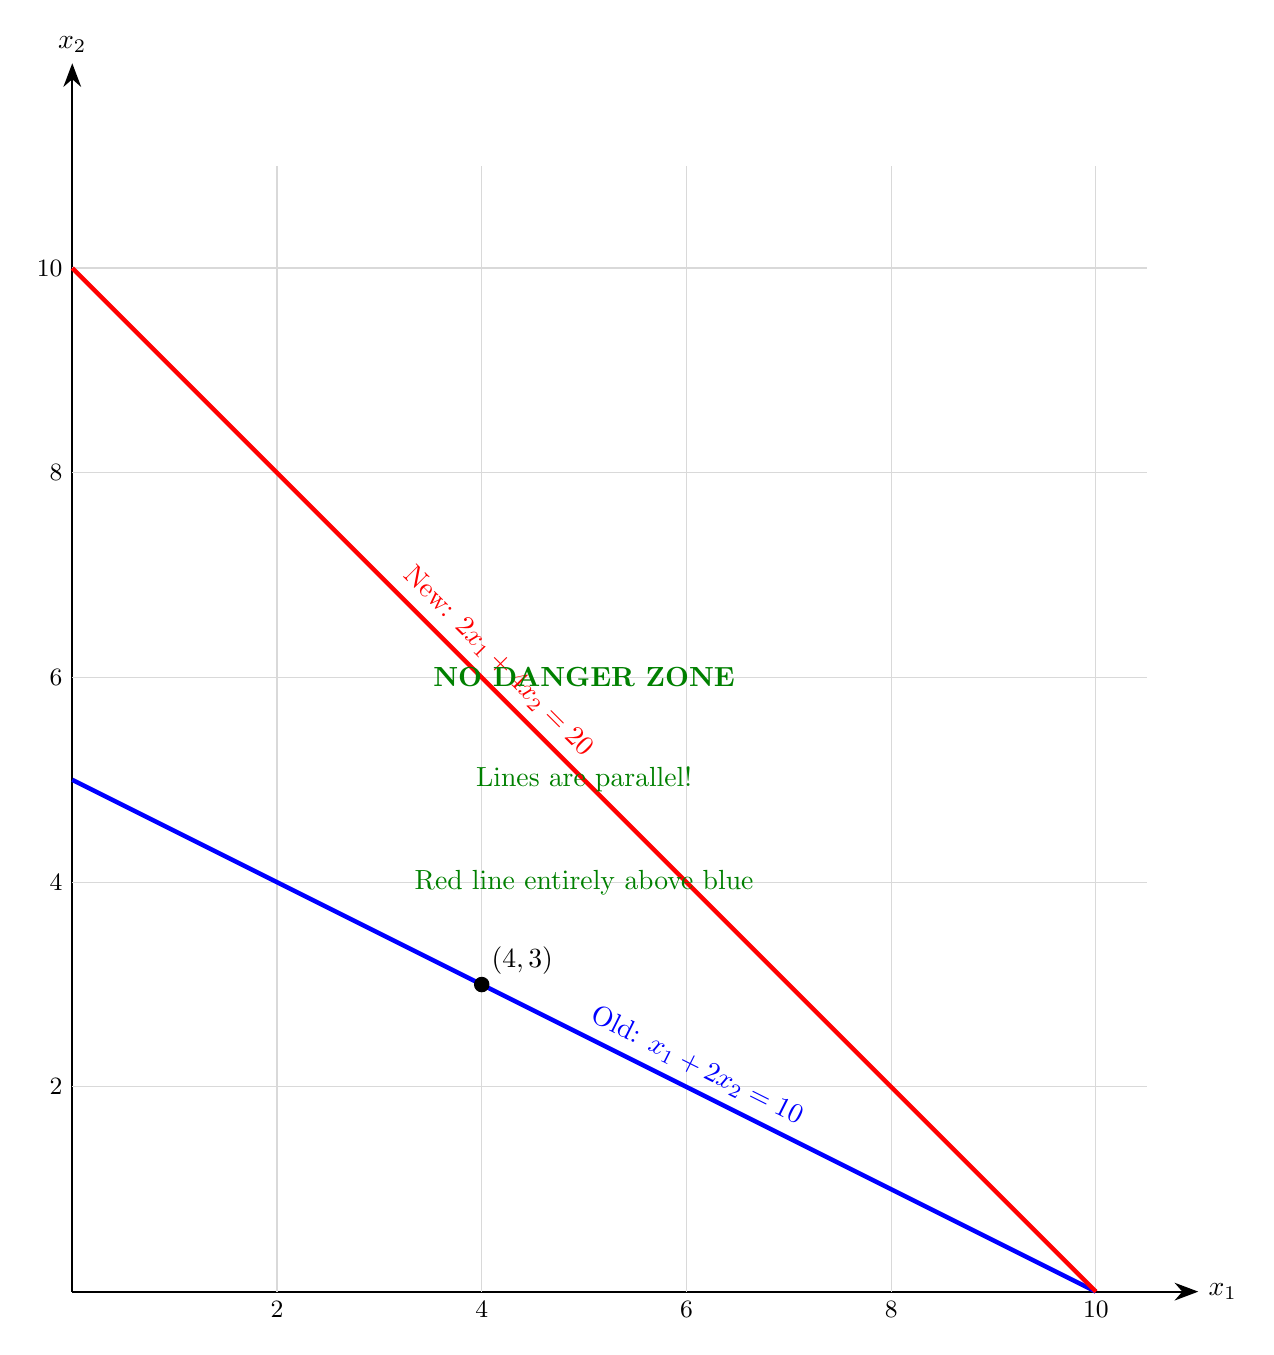
\begin{tikzpicture}[scale=1.3]
    \draw[-{Stealth[length=3mm]},thick] (0,0) -- (11,0) node[right] {$x_1$};
    \draw[-{Stealth[length=3mm]},thick] (0,0) -- (0,12) node[above] {$x_2$};

    \foreach \x in {2,4,6,8,10}
        \draw[gray!30] (\x,0) -- (\x,11);
    \foreach \y in {2,4,6,8,10}
        \draw[gray!30] (0,\y) -- (10.5,\y);

    \draw[blue, ultra thick] (0,5) -- (10,0) node[pos=0.6,above,sloped,blue] {Old: $x_1 + 2x_2 = 10$};
    \draw[red, ultra thick] (0,10) -- (10,0) node[pos=0.4,above,sloped,red] {New: $2x_1 + 4x_2 = 20$};

    % These lines are PARALLEL! (same slope -1/2)
    % Red line is above blue line everywhere
    % No intersection in positive quadrant

    \filldraw[black] (4,3) circle (2pt) node[above right] {$(4,3)$};

    \node[green!50!black, font=\bfseries] at (5,6) {NO DANGER ZONE};
    \node[green!50!black] at (5,5) {Lines are parallel!};
    \node[green!50!black] at (5,4) {Red line entirely above blue};

    \foreach \x in {2,4,6,8,10}
        \node[below] at (\x,0) {\small \x};
    \foreach \y in {2,4,6,8,10}
        \node[left] at (0,\y) {\small \y};
\end{tikzpicture}
\end{center}

\textbf{Characteristics:}
\begin{itemize}
\item The lines are \textbf{parallel} (same slope)
\item New iso-cost line is entirely \textbf{above} old budget line
\item No intersection = No danger zone
\item \textbf{Every bundle is safe!}
\item This happens when all prices change by the same proportion (multiply by constant)
\end{itemize}

\textbf{Economic interpretation:} If all prices double, any bundle you buy reveals your current budget is 2× whatever it was. But that doesn't create a WARP violation because the affordability sets don't overlap properly.

\newpage

\section{Scenario 4: Entire Region is Danger Zone}

\textbf{Setup:}
\begin{itemize}
\item Old prices: $(2, 3)$, bought $(5, 0)$, budget = 10
\item New prices: $(1, 5)$, old bundle costs 5
\item Price of good 1 \textbf{decreased}, price of good 2 \textbf{increased}
\end{itemize}

\begin{center}
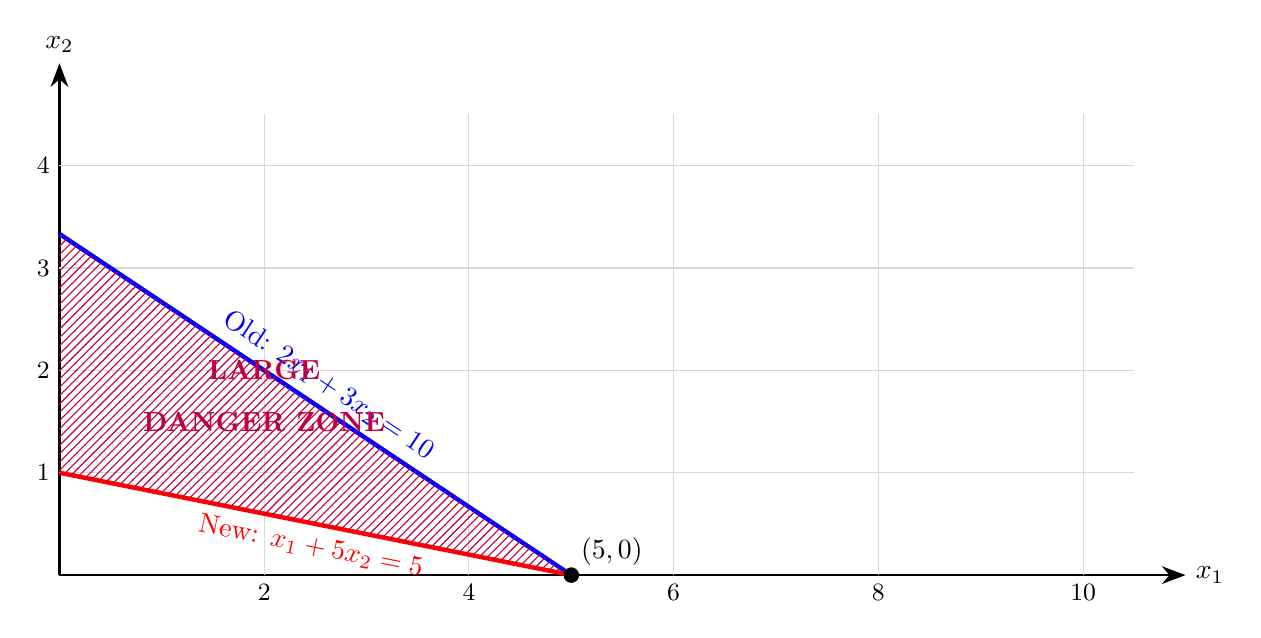
\begin{tikzpicture}[scale=1.3]
    \draw[-{Stealth[length=3mm]},thick] (0,0) -- (11,0) node[right] {$x_1$};
    \draw[-{Stealth[length=3mm]},thick] (0,0) -- (0,5) node[above] {$x_2$};

    \foreach \x in {2,4,6,8,10}
        \draw[gray!30] (\x,0) -- (\x,4.5);
    \foreach \y in {1,2,3,4}
        \draw[gray!30] (0,\y) -- (10.5,\y);

    \draw[blue, ultra thick] (0,3.333) -- (5,0) node[pos=0.5,above,sloped,blue] {Old: $2x_1 + 3x_2 = 10$};
    \draw[red, ultra thick] (0,1) -- (5,0) node[pos=0.5,below,sloped,red] {New: $x_1 + 5x_2 = 5$};

    % Red line (new) is BELOW blue line (old)
    % Danger zone: below blue AND above red
    % This is the region between the two lines

    \fill[pattern=north east lines, pattern color=purple] (0,1) -- (5,0) -- (0,3.333) -- cycle;

    \filldraw[black] (5,0) circle (2pt) node[above right] {$(5,0)$};

    \node[purple, font=\bfseries] at (2,2) {LARGE};
    \node[purple, font=\bfseries] at (2,1.5) {DANGER ZONE};

    \foreach \x in {2,4,6,8,10}
        \node[below] at (\x,0) {\small \x};
    \foreach \y in {1,2,3,4}
        \node[left] at (0,\y) {\small \y};
\end{tikzpicture}
\end{center}

\textbf{Characteristics:}
\begin{itemize}
\item Large triangular danger zone
\item Original bundle is on the boundary (corner solution at $(5,0)$)
\item New iso-cost line is \textbf{below} old budget line
\item Most of what was affordable before creates violations
\item This happens when: good 1 gets cheaper, good 2 gets more expensive, and you were buying only good 1
\end{itemize}

\textbf{Why this is large:} Since the new bundle (5,0) costs only \$5 at new prices, buying almost anything costs $\geq$ \$5, so most old affordable bundles create violations!

\newpage

\section{Summary Table}

\begin{center}
\begin{tabular}{|p{3cm}|p{4cm}|p{4cm}|p{3cm}|}
\hline
\textbf{Scenario} & \textbf{Relative Slopes} & \textbf{Danger Zone Shape} & \textbf{Touches} \\
\hline
Classic Triangle & Old steeper than new & Triangle below & $x_1$-axis \\
\hline
Flipped Triangle & Old flatter than new & Triangle on left & $x_2$-axis \\
\hline
No Danger Zone & Parallel lines (proportional prices) & None / Empty & Nothing \\
\hline
Large Zone & New line below old & Large triangle & Both axes \\
\hline
\end{tabular}
\end{center}

\section{Key Insights}

\begin{enumerate}
\item The danger zone is \textbf{not always a triangle touching the x-axis}!

\item The shape depends on:
\begin{itemize}
\item Which price increased more (relative to the other)
\item The original bundle's composition
\item Whether prices changed proportionally
\end{itemize}

\item The danger zone can:
\begin{itemize}
\item Touch $x_1$-axis (when old budget steeper)
\item Touch $x_2$-axis (when new iso-cost steeper)
\item Not exist at all (parallel lines)
\item Be very large (when new line below old)
\end{itemize}

\item \textbf{General rule:} The danger zone exists when the two lines intersect in the positive quadrant, and it's the region satisfying BOTH constraints.
\end{enumerate}

\end{document}
